%%% Copyright (C) 2020 David Beauchemin
%%%
%%% Ce fichier et tous les fichiers .tex dont la racine est
%%% mentionnée dans les commandes \include et \input ci-dessous font
%%% partie du projet «Reproductibilité en apprentissage automatique
%%% - Webinaire de l'AAIARD»
%%% https://davebulaval.github.io/reproductibilite-en-apprentissage-automatique/
%%%
%%% Le format et le visuel est très fortement inspiré du matériel de
%%% Vincent Goulet https://gitlab.com/vigou3/webinaire-recherche-reproductible
%%%
%%% Cette création est mise à disposition selon le contrat
%%% Attribution-Partage dans les mêmes conditions 4.0
%%% International de Creative Commons.
%%% https://creativecommons.org/licenses/by-sa/4.0/

\documentclass[aspectratio=169,10pt,xcolor=x11names,english,french]{beamer}
\usepackage{babel}
\usepackage[autolanguage]{numprint}
\usepackage{amsmath}
\usepackage{currfile}                  % nom fichier de script
\usepackage{changepage}                % page licence
\usepackage{tabularx}                  % page licence
\usepackage{relsize}                   % \smaller et al.
\usepackage{awesomebox}                % boites signalétiques
\usepackage{fancyvrb}                  % texte verbatim
\usepackage{framed}                    % env. leftbar
\usepackage{pict2e}                    % cycle travail Git
\usepackage[overlay,absolute]{textpos} % couvertures
\usepackage{metalogo}       
\usepackage{textpos}           % logo \XeLaTeX

\usepackage{booktabs}

\usepackage{fontawesome}

\usepackage{pgfplots}
\usepackage{pgfplotstable}

\usepackage{stackengine} % for stacking logo
\usepackage{tikz}
\usetikzlibrary{decorations.pathreplacing}
\usetikzlibrary{fadings}
\usetikzlibrary{positioning} %for lstm
\usetikzlibrary{shapes, backgrounds}
\usetikzlibrary{arrows}
\usetikzlibrary{chains}
\tikzstyle{line} = [draw, -latex']
\usetikzlibrary{calc}

\usepackage{svg} %for svg image also need option --shell-escape

%% =============================
%%  Informations de publication
%% =============================
\title{Reproductibilité en apprentissage automatique}
\author{David Beauchemin}
\date{30 octobre 2020}

%% =======================
%%  Apparence du document
%% =======================

%% Couleurs additionnelles
\definecolor{rouge}{rgb}{1,0.31,0.26}
\definecolor{bleu}{rgb}{0.18,0.23,1}
\definecolor{couleurpolice}{rgb}{0.13,0.13,0.13}

\definecolor{link}{cmyk}{0.67, 0.66, 0, 0.71}    % liens internes
\definecolor{url}{rgb}{1,0.31,0.26}       % liens externes
\definecolor{codebg}{rgb}{0.94, 0.95, 0.95}

\colorlet{shadecolor}{codebg}

%% Thème Beamer général
\usetheme[titleformat=allcaps, numbering=none, block=transparent]{metropolis}

%% Modifications aux couleurs: fond blanc, titres en texte noir sur
%% fond blanc
\setbeamercolor{normal text}{bg=white}
\setbeamercolor{frametitle}{fg=normal text.fg, bg=}

%% Déplacer les titres vers le bas sous la décoration du gabarit CFDD
\makeatletter
\setlength{\metropolis@frametitle@padding}{4.9ex}
\renewcommand{\metropolis@frametitlestrut@start}{
	\rule{0pt}{6ex +%
		\totalheightof{%
			\ifcsdef{metropolis@frametitleformat}{\metropolis@frametitleformat X}{X}%
		}%
	}
}
\renewcommand{\metropolis@frametitlestrut@end}{}
\makeatother

%% Format de la page de titre de section;
\makeatletter

\setbeamertemplate{section page}{%
	\begin{minipage}{40em}
		\raggedright
		\usebeamerfont{section title}
		\let\hyperlink\@secondoftwo\fontsize{35}{35}\textcolor[cmyk]{0.67, 0.66, 0, 0.71}{\insertsectionhead}\par
		\note{}
	\end{minipage}
	\par
	\vspace{\baselineskip}
}

\makeatother

%% Polices de caractères
\newfontfamily\Overpass{Overpass}
\setsansfont{Overpass}        % police principale
\newfontfamily\OverpassSemiBold{Overpass}
[
BoldFont = *-SemiBold
]
\newfontfamily\OverpassExtraLightBold{Overpass}
[
UprightFont = *-ExtraLight,
BoldFont = *-Light
]
\newfontfamily\OverpassLight{Overpass}
[
UprightFont = *-Light,
BoldFont = *-Regular
]


\setbeamercolor{frametitle}{fg=couleurpolice}
\setbeamercolor{section in head/foot}{fg=couleurpolice}
\setbeamercolor{normal text}{fg=couleurpolice}



%% Hyperliens
\hypersetup{%
	pdfauthor = {David Beauchemin},
	pdftitle = {Gestion de la configuration et des résultats avec MLflow, Hydra et Poutyne},
	colorlinks = {true},
	linktocpage = {true},
	allcolors = {link},
	urlcolor = {url},
	pdfpagemode = {UseOutlines},
	pdfstartview = {Fit},
	bookmarksopen = {true},
	bookmarksnumbered = {true},
	bookmarksdepth = {subsection}}

%% Paramétrage de babel pour les guillemets
\frenchbsetup{og=«, fg=»}

%% =========================
%%  Nouveaux environnements
%% =========================

%% Environnement pour le code informatique; hybride
%% des environnements snugshade* et leftbar de framed.
\makeatletter
\newenvironment{Scode}{%
	\def\FrameCommand##1{\hskip\@totalleftmargin
		\vrule width 3pt\colorbox{codebg}{\hspace{5pt}##1}%
		% There is no \@totalrightmargin, so:
		\hskip-\linewidth \hskip-\@totalleftmargin \hskip\columnwidth}%
	\MakeFramed {\advance\hsize-\width
		\@totalleftmargin\z@ \linewidth\hsize
		\advance\labelsep\fboxsep
		\@setminipage}%
}{\par\unskip\@minipagefalse\endMakeFramed}
\makeatother

%% Environnement pour le contenu d'un fichier; alias de snugshade*.
\newenvironment{Sfile}{\begin{snugshade*}}{\end{snugshade*}}

%% =====================
%%  Nouvelles commandes
%% =====================

%% Lien externe
\newcommand{\link}[2]{\href{#1}{#2~{\smaller\faExternalLink*}}}
\newcommand{\email}[2]{\href{#1}{#2~{\smaller\faInbox*}}}
\newcommand{\guillemet}[1]{\guillemotleft #1 \guillemotright}

%% Simili commande \HUGE
\newcommand{\HUGE}{\fontsize{36}{36}\selectfont}

%%% =======
%%%  Varia
%%% =======

%% Longueurs pour la composition des pages couvertures avant et
%% arrière
\newlength{\banderougewidth} \newlength{\banderougeheight}
\newlength{\bandeorwidth}    \newlength{\bandeorheight}
\newlength{\imageheight}     \newlength{\imagewidth}
\newlength{\logoheight}

\newcounter{frame}[frame]
\setbeamertemplate{footline}[frame number] 

\begin{document}
	
	%% Style de l'entête et du pied de page
	
	%% frontmatter
	%%% Copyright (C) 2020 David Beauchemin
%%%
%%% Ce fichier et tous les fichiers .tex dont la racine est
%%% mentionnée dans les commandes \include et \input ci-dessous font
%%% partie du projet «Reproductibilité en apprentissage automatique
%%% - Webinaire de l'institut intelligence et données»
%%% URL
%%%
%%% Le format et le visuel est très fortement inspiré du matériel de
%%% Vincent Goulet https://gitlab.com/vigou3/webinaire-recherche-reproductible
%%%
%%% Cette création est mise à disposition selon le contrat
%%% Attribution-Partage dans les mêmes conditions 4.0
%%% International de Creative Commons.
%%% https://creativecommons.org/licenses/by-sa/4.0/

%% Normes de présentation visuelle 2018
%%
%% - grille de 8 unités de haut
%% - 1 mesure = 1/8 d'unité
%% - bande identitaire de 1 mesure placée au bas de la 7e unité
%% - logo haut de 4 mesures avec blancs de deux mesures en haut et
%%   en bas
%% - blanc équivalent à la largeur du blason à droite du logo
%% - bande or de la largeur du logo + blanc à droite
%%
%% Dimensions du logo UL
%%
%% hauteur: 129
%% largeur totale: 312
%% largeur blason: 102
%% valeur clé: (312 + 102)/129 = 3.209302
%%
%% Dimensions de l'image
%%
%% hauteur: 55 mesures - 1pt (filet) = 54.9191919 mesures
%% largeur: 160mm
%% ratio largeur/hauteur: 160/77.23

\begingroup
\TPGrid{16}{64}
\textblockorigin{0mm}{0mm}
\setlength{\parindent}{0mm}
\setlength{\imageheight}{54.9191919\TPVertModule}
\setlength{\logoheight}{4\TPVertModule}
\setlength{\bandeorwidth}{3.209302\logoheight}
\setlength{\banderougewidth}{\paperwidth}
\addtolength{\banderougewidth}{-\bandeorwidth}
\setlength{\bandeorheight}{\TPVertModule}
\setlength{\banderougeheight}{\TPVertModule}
\setlength{\textwidth}{\paperwidth}
\addtolength{\textwidth}{-2\TPHorizModule}

\def\titlefmt{%
  \bfseries\fontsize{24}{24}\selectfont%
  DETECTION OF DUPLICATES AMONG NON-STRUCTURED DATA FROM DIFFERENT DATA SOURCES\par}

\def\fsgiid{%
	\OverpassLight\fontsize{4.5}{4.5}\selectfont%
	\bfseries\textcolor{black}{Faculté des sciences et de génie} \\
	\mdseries\textcolor[gray]{0.35}{Institut Intelligence et Données (IID)}}

\def\iidurl{%
	\OverpassLight\fontsize{4.5}{4.5}\selectfont%
	\bfseries\textcolor{black}{iid.ulaval.ca}}


%%%
%%% Page de titre
%%%
\begin{frame}[plain]
  %% bandeau identitaire
  \begin{textblock*}{\paperwidth}[0,1](0mm,56\TPVertModule)
    \textcolor{rouge}{\rule{\banderougewidth}{\banderougeheight}}% % bande rouge
    \textcolor{or}{\rule{\bandeorwidth}{\bandeorheight}}           % bande or
  \end{textblock*}

  %% logo UL
  \begin{textblock*}{\bandeorwidth}(\banderougewidth,58\TPVertModule)
    
\includegraphics[height=\logoheight,keepaspectratio=true]{%
      img/ul_p.pdf}
  \end{textblock*}
  \begin{textblock*}{3\TPHorizModule}[1,0.5](14\TPHorizModule,59.7\TPVertModule)
    \raggedleft\fsgiid
  \end{textblock*}
  \begin{textblock*}{3\TPHorizModule}[0,0.5](0.7\TPHorizModule,59.7\TPVertModule)
		\iidurl
	\end{textblock*}

  %% titre
  \begin{textblock*}{10\TPHorizModule}(0.7\TPHorizModule,17\TPVertModule)
    \textcolor[cmyk]{0.67, 0.66, 0, 0.71}{\titlefmt}
  \end{textblock*}

\end{frame}
\endgroup

	
	\begin{frame}
		\frametitle{About myself}
		
		\begin{minipage}{0.25\linewidth}
			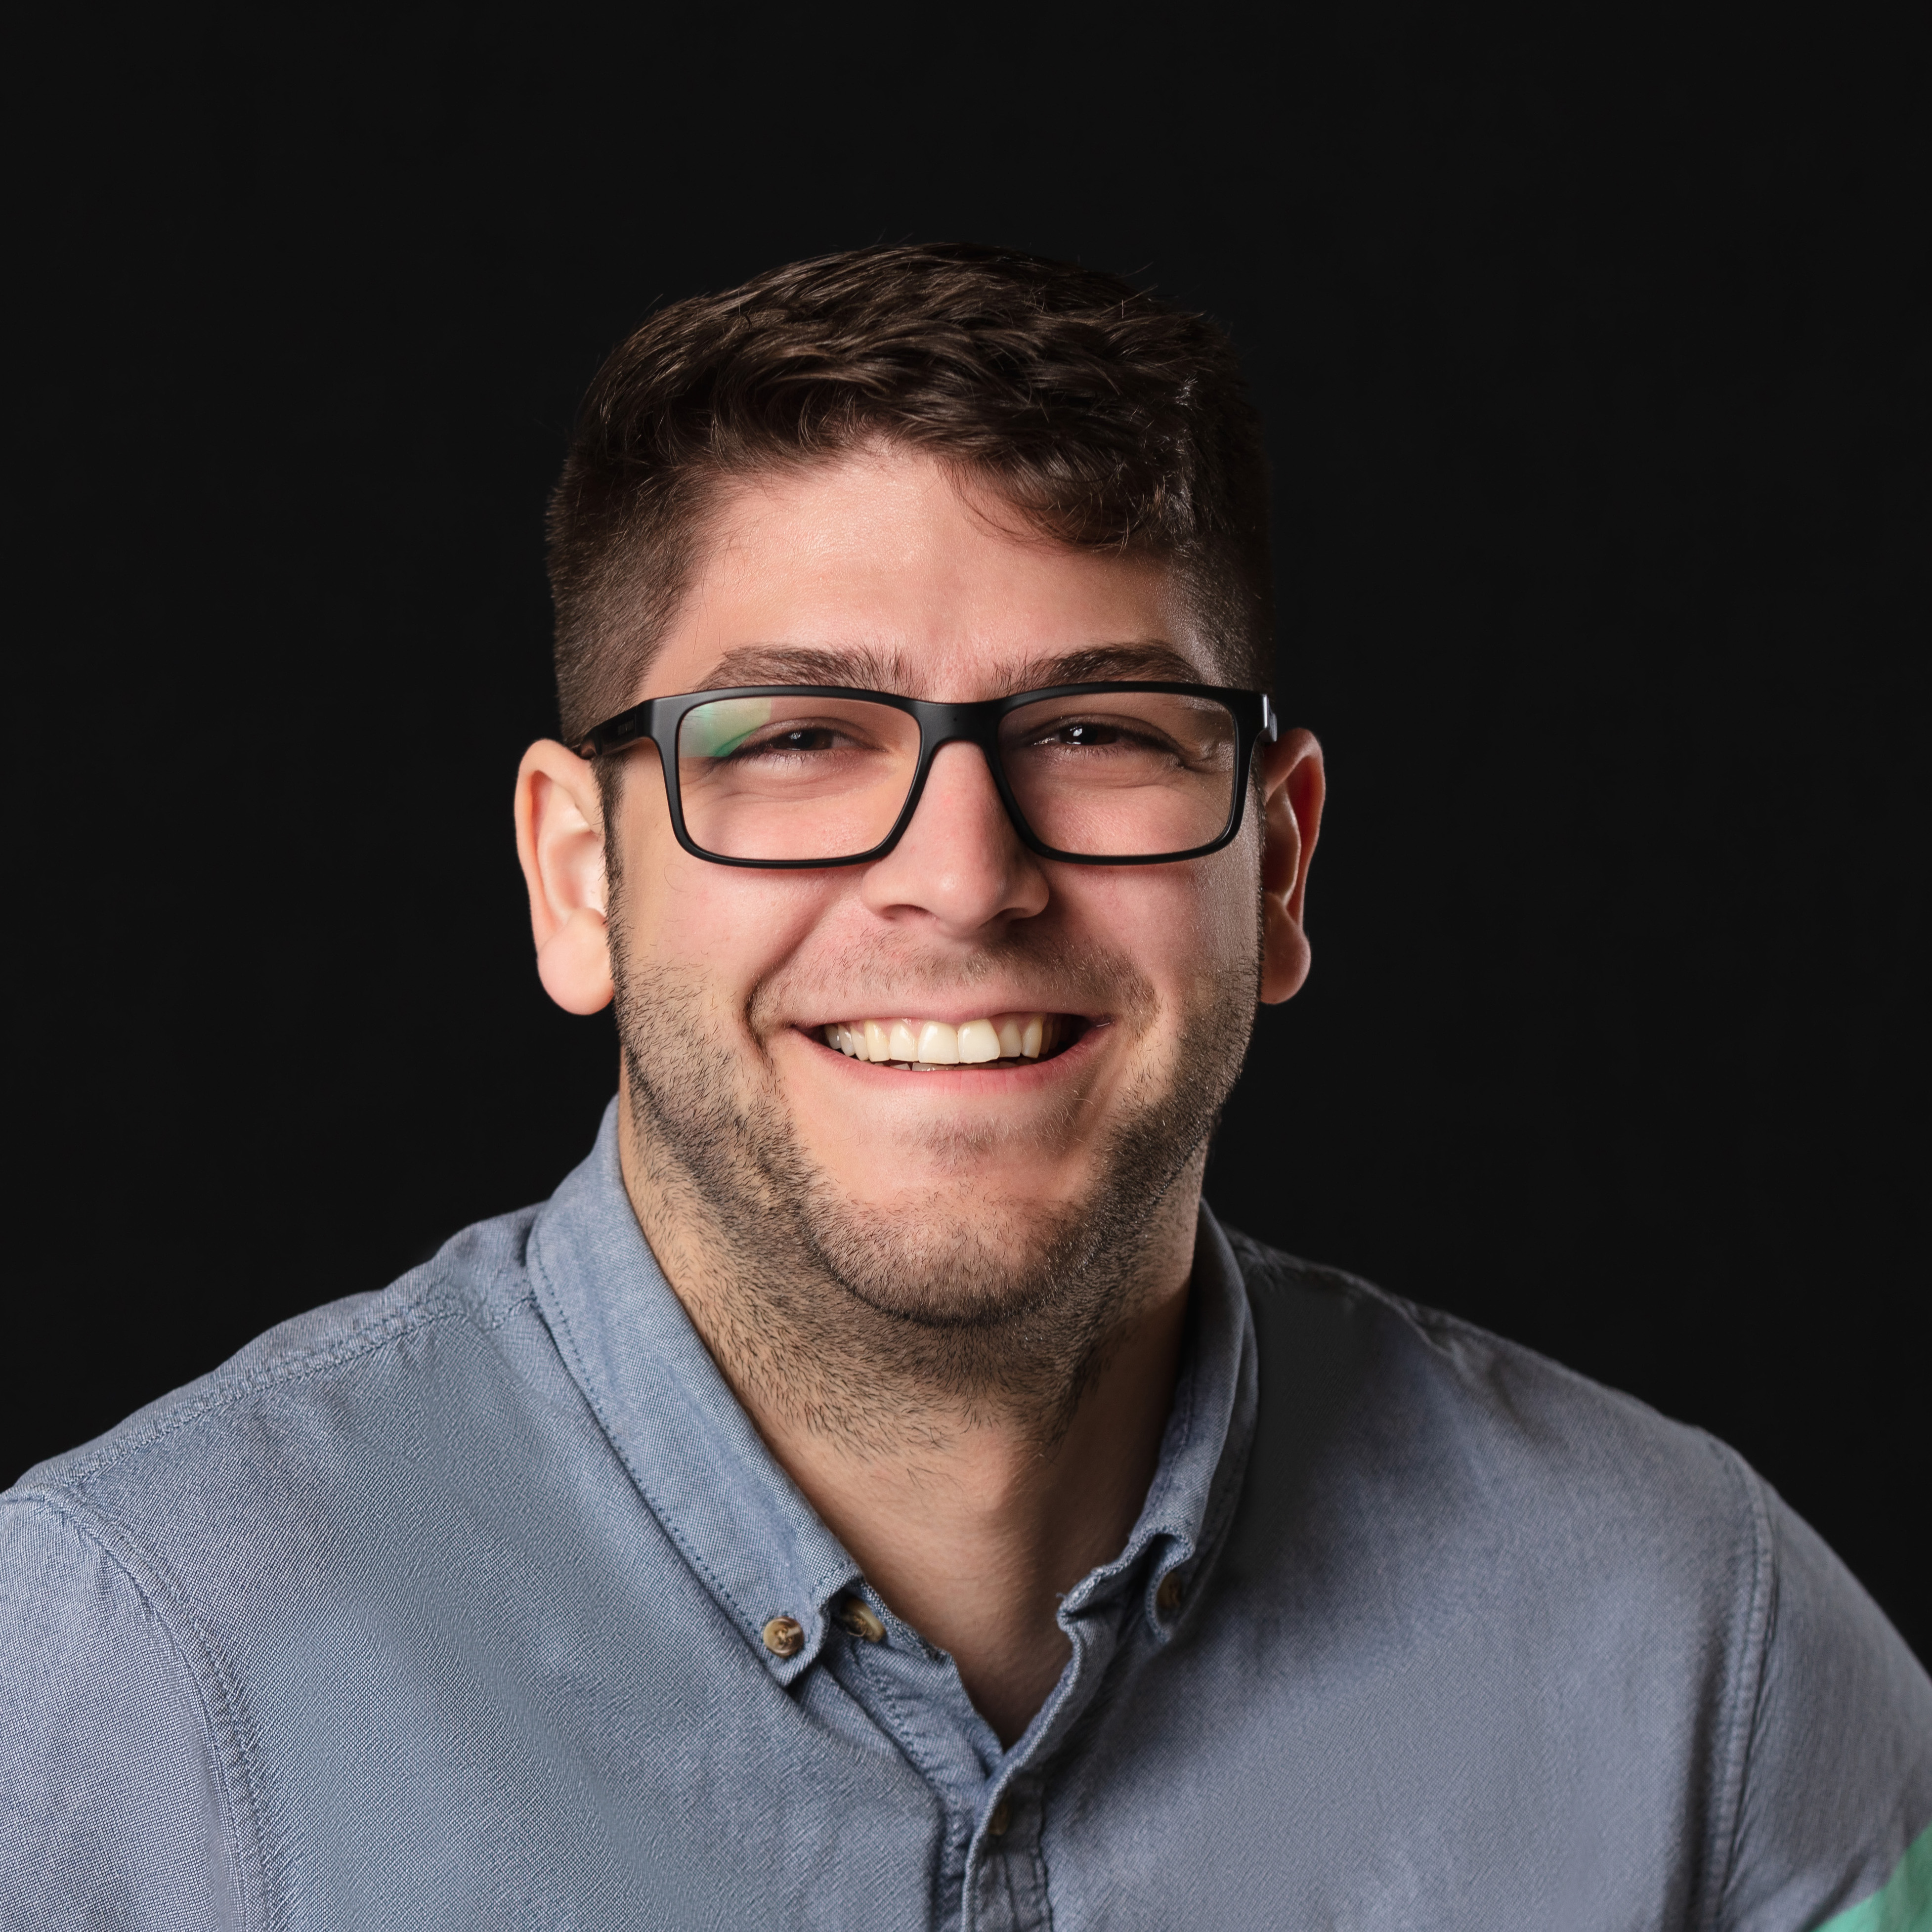
\includegraphics[width=\linewidth,keepaspectratio]{img/david}
		\end{minipage}
		\hfill
		\begin{minipage}{0.70\linewidth}
			\begin{itemize}
				\item B. Sc. in actuarial science
				\item M. Sc. in computer science, ML and NLP
				\item 5 years in academic ML and NLP researc project
				\item +6 years of various applied business projects
				\item Founder and creator of \link{https://anchor.fm/open-layer}{OpenLayer} a bilingual AI podcast
				\item Founder of \link{https://www.dotlayer.org/}{.Layer} a data science non-profit organisation
			\end{itemize}
		\end{minipage}
		
		\begin{minipage}{0.25\linewidth}
			\small
			\textbf{DAVID BEAUCHEMIN} \\
			Ph. D. candidate in ML\\
			\footnotesize Laval University
		\end{minipage}
		\note{
			À lire
		}
	\end{frame}

	\begin{frame}{Menu}
		\begin{enumerate}
			\item What is our problem?
			\item How can we develop a solution for that?
			\item How can we compute the similarity between two entities?
			\item Why develop our own solutions?
		\end{enumerate}
	\end{frame}
	\section{What is our problem?}
	\begin{frame}{What is our problem?}
  		\begin{minipage}{\linewidth}
			\centering
			\fontsize{35}{35}\faDollarSign \vfil
			\vspace{1em}
			\normalsize Data is not cheap
		\end{minipage}
		\note{You may have heard plenty of times that data is the new oil. But oil, thus data, is not cheap. And we are in a time where we need to move fast; therefore cannot always properly create new in-house datasets for our needs.}
	\end{frame}

	\begin{frame}{What is our problem?}
		\begin{minipage}{\linewidth}
			\centering
			\fontsize{35}{35}\faBoxOpen \vfil
			\vspace{1em}
			\normalsize A lot of open data now (\link{https://data.gov/}{data.gouv})
		\end{minipage}
		\note{Moreover, with the rise of public datasets curated by large public organizations such as censuses (WHO) and various government, state and cities public datasets, it becomes more and more interesting to use those open datasets.}
	\end{frame}

	\begin{frame}{What is our problem?}
		\begin{minipage}{\linewidth}
			\centering
			\fontsize{35}{35}\faCodeBranch \vfil
			\vspace{1em}
			\normalsize Mapping between datasets
		\end{minipage}
		\note{However, a problem arises when trying to use various open data with our private data, that is, mapping data points between different sources.}
	\end{frame}

	\begin{frame}{An example}
		Only using the name and the address of a business client is it possible to match these with external sources to leverage their content?
		\note{I will use a use case example for the rest of this presentation. It is based on my master thesis work with an insurance company interested in using external sources to lower the number of questions in a risk assessments to compute is premium.}
	\end{frame}

	\begin{frame}{An example}
		\begin{center}
			\begin{tikzpicture}[internal/.style={draw, rectangle, minimum width=4cm, inner sep=4pt},
				every text node part/.style={align=center}]

				\node (node1) at (0, 0) [cylinder, shape border rotate=90, draw, minimum height=1.25cm, minimum width=2.5cm, aspect=0.2] {Opencorporates};
				\node[above=0.5cm of node1]  (node2) [cylinder, shape border rotate=90, draw, minimum height=1.25cm, minimum width=2.5cm, aspect=0.2] {Yelp};
				\node[below=0.5cm of node1] (node3) [cylinder, shape border rotate=90, draw, minimum height=1.25cm, minimum width=2.5cm, aspect=0.2] {Opencorpdata};
				
				\node[left=2cm of node1] (node4) [internal, shape border rotate=90, draw, minimum height=1.15cm,minimum width=2cm, aspect=0.2] {Sirius Cybernetics Corp.\\ 221B Baker St., London};
				\draw [-stealth, line width=1mm] (node4) -- node[sloped, anchor=center, above] {} (node1);
				\draw [-stealth, line width=1mm] (node4) -- node[sloped, anchor=center, above] {} (node2);
				\draw [-stealth, line width=1mm] (node4) -- node[sloped, anchor=center, above] {} (node3);
				\draw [decorate,decoration={brace,amplitude=12pt},xshift=-4pt,yshift=-6pt, line width=1mm] (-7.5,3.25) -- (1.25,3.25) node [black,midway,yshift=+1cm]{Is this data point in\\one of these sources?};
				
			\end{tikzpicture}
		\end{center}
		\note{Let use an example to further illustrate our problem. Let say we have a client database with business names and address and we would like to levrage external data sources to extract more information of those clients without the need to speak with them.}
	\end{frame}

	\begin{frame}{An example}
		How can we match our information with external data sources if we do not control it and our information is not unique?
		\note{A question arises from the example, how can we match data that is not unique? Names are definitely not unique, and addresses are not "unique," but clients can change over time; thus a given address can appear multiple times in a dataset.}
	\end{frame}
	
	\section{How can we develop a solution for that?}
	
	\begin{frame}{What our solution needs to do?}
	\begin{center}
		\begin{tikzpicture}[internal/.style={draw, rectangle, minimum width=4cm, inner sep=4pt},
			every text node part/.style={align=center}]
			\node[internal, align=center, minimum height=1.15cm](node1) at (-5, -2.75) {Our solution};
			
			\node (node2) at (0, -2.75) [cylinder, shape border rotate=90, draw, minimum height=1.15cm, minimum width=2cm, aspect=0.2] {Opencorporates};
			\draw[->,>=stealth, line width=1mm] (node2) edge (node1.east);
			
			\node (node3) at (-10, -2.75) [cylinder, shape border rotate=90, draw, minimum height=1.15cm,minimum width=2cm, aspect=0.2] {Our database};
			\draw[->,>=stealth, line width=1mm] (node3) edge (node1.west);
			
			\node[internal, align=center, rounded corners=1ex, minimum height=1.15cm](node4) at (-5, -5.5) {Sirius Cybernetics\\221B Baker St., Montreal};
			%\node[internal, align=center, rounded corners=1ex, minimum height=1.15cm, fill=white](node5) at (-5.25, -5.75) {\\};
			\node[internal, align=center, rounded corners=1ex, minimum height=1.15cm, fill=white](node6) at (-5.50, -6) {Sirius Cybernetics Corp.\\ 221B Baker St., London};
			
			\draw[->,>=stealth, line width=1mm] (node1) edge (node4);
		\end{tikzpicture}
	\end{center}
	\note{Our solution needs to be able to take at least two databases and extract the duplicate element among the two data sources. Namely, duplicate detection. That is, detecting if two data points are duplicates or not.}
	\end{frame}

	\begin{frame}{What do we need to achieve that?}
		\begin{itemize}
			\item Natural language processing (NLP)
			\item A duplicate detection mechanism
		\end{itemize}
		\note{To achieve such a solution, we need to use NLP and use or develop a duplicate detection mechanism that will be able to match duplicate records between sources.}
	\end{frame}

	\begin{frame}{What is NLP?}
		\begin{center}
			\begin{tikzpicture}[thick,
				set/.style = {circle,
					minimum size = 3cm}]
				
				% Set A
				\node[set,label={135:CS}, fill=rouge!30] (A) at (0,0) {};
				
				% Set B
				\node[set,label={45:AI}, fill=bleu!30] (B) at (1.8,0) {};
				
				% Set C
				\node[set,label=Linguistics, fill=couleurpolice!30] (C) at (0.9,1.5) {};
				
				% Intersection
				\begin{scope}
					\clip (0,0) circle(1.5cm);
					\clip (1.8,0) circle(1.5cm);
					\clip (0.9,1.5) circle(1.5cm);
					\fill[orange!60](0,0) circle(1.5cm);
				\end{scope}
				
				% Circles outline
				\draw (0,0) circle(1.5cm);
				\draw (1.8,0) circle(1.5cm);
				\draw (0.9,1.5) circle(1.5cm);
				\node at (barycentric cs:A=1,B=1 ,C=1) {NLP};
				
			\end{tikzpicture}
		\end{center}
		\note{So first, what we need is NLP. So, let's first define what NLP is.
			NLP is a subfield of linguistics, computer science, and artificial intelligence concerned with the interactions between computers and human language, in particular how to program computers to process and analyze large amounts of natural language data. 
			
			Thus, we need NLP because the data we can use to identify two similar data points will most likely be textual data such as clients' names, addresses, and customer reviews. Otherwise, if we have numerical data such as social security numbers or any numerical data that is a unique mapping to a client, we do not require duplicate detection but rather classical programming rules.}
	\end{frame}

	\begin{frame}{What is AI?}
		\begin{center}
			\center
			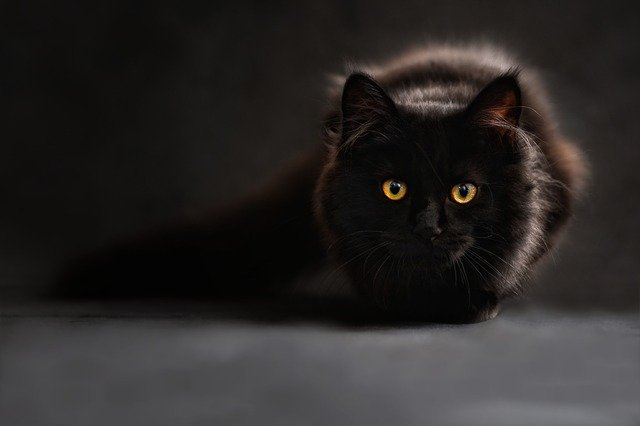
\includegraphics[scale=0.25, keepaspectratio]{img/cat}
			
			A cat or not?
		\end{center}
		\note{I will not argue about the definition of intelligence or AI. For this presentation, when I say AI, what I mean is machine learning -> ML and, more precisely, supervised ML. The basic idea of ML is to develop a system that can, given data, statistically predict something. For example, let's say we want to classify if a picture includes a cat. A non-AI system will use heuristic rules such as: does it have fur, claws, etc.}
	\end{frame}

	\begin{frame}{What is AI?}
		\centering
		\begin{tikzpicture}[internal/.style={draw, rectangle, inner sep=4pt},
			every text node part/.style={align=center}]
			\node(node1) at (0, 0) {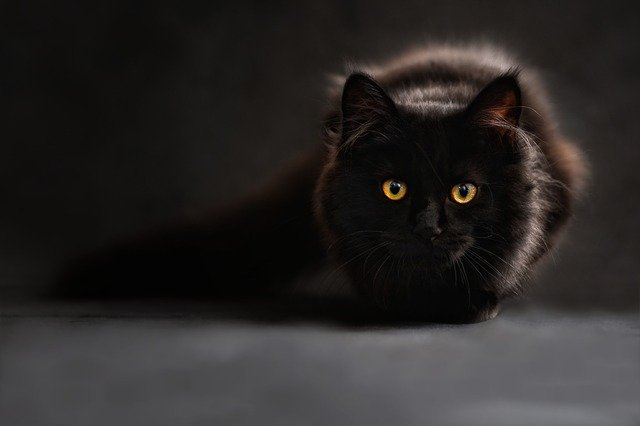
\includegraphics[scale=0.15, keepaspectratio]{img/cat}};
			\node[align=center, below right=5mm of node1](label) {``A cat"};
			
			\node[internal, align=center, minimum height=1.15cm, right=1cm of node1](node2) {ML Model};
			
			\draw[->,>=stealth, line width=1mm] (node1) edge (node2);
			\draw[->,>=stealth, line width=1mm] (label) edge (node2);
				
			\node[align=center, right=1cm of node2](node3) {``Not a cat"};
			\draw[->,>=stealth, line width=1mm] (node2) edge (node3);
			
		\end{tikzpicture}
		\note{Where an ML approach will use numerous labelled data of cats that include or not a cat and will try to learn his own representation of a cat, where the label are used to give insight to the model where he is mistaken.}
	\end{frame}

	\begin{frame}{What is AI?}
		\centering
		\begin{tikzpicture}[internal/.style={draw, rectangle, inner sep=4pt},
			every text node part/.style={align=center}]
			\node(node1) at (0, 0) {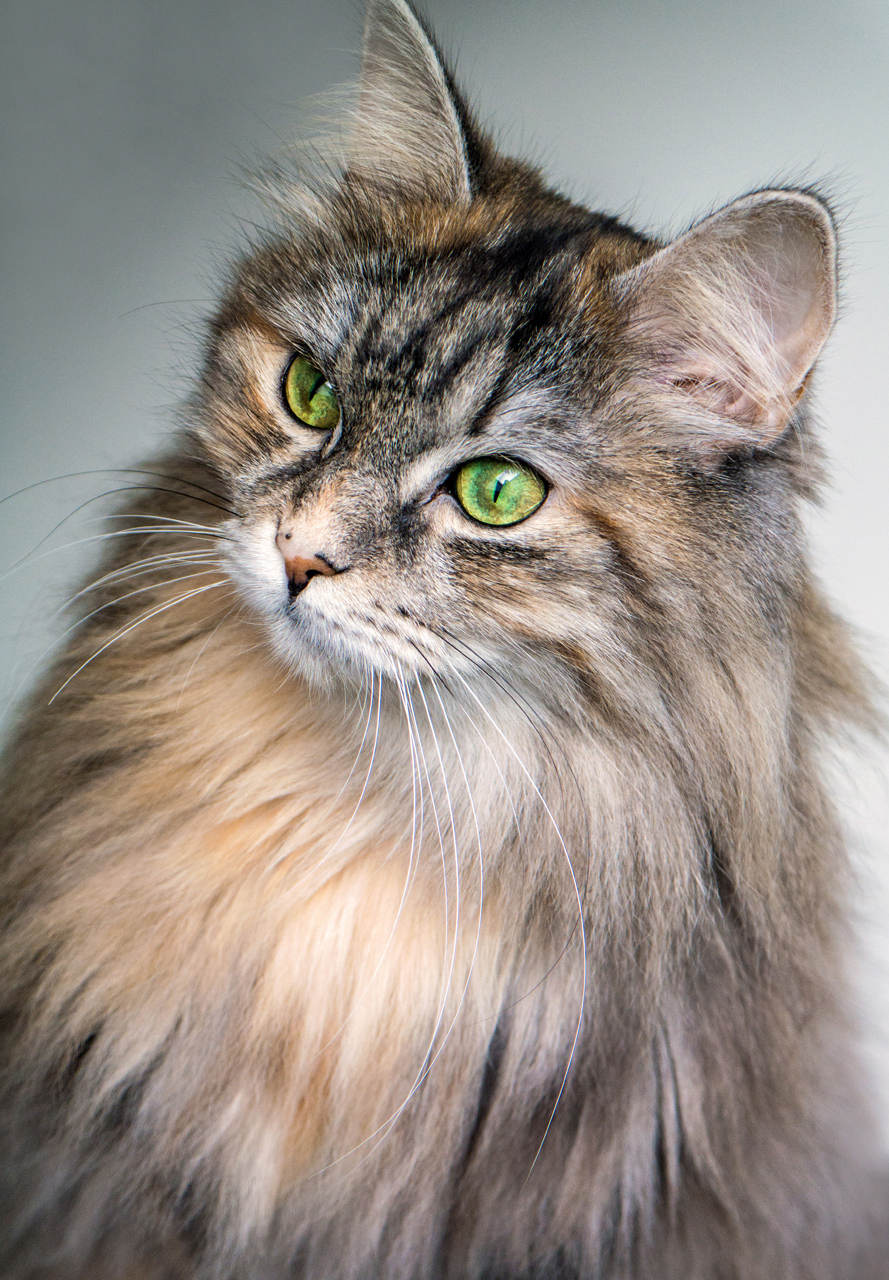
\includegraphics[scale=0.25, keepaspectratio]{img/cat_2}};
			%\node[internal, align=center, below right=5mm of node1](label) {``cat"};
			
			\node[internal, align=center, minimum height=1.15cm, right=1cm of node1](node2) {ML Model};
			
			\draw[->,>=stealth, line width=1mm] (node1) edge (node2);
			%				\draw[->,>=stealth, line width=1mm] (label) edge (node2);
			
			\node[align=center, right=1cm of node2](node3) {``cat"};
			\draw[->,>=stealth, line width=1mm] (node2) edge (node3);
			
		\end{tikzpicture}
		\note{and use those internal representations to predict never seen picture. So, in brief, the basic idea of supervised ML is to teach a model or something by giving it examples of the expected output given a context (the image) using labelled examples.}
	\end{frame}

	\begin{frame}\frametitle{duplicate detection mechanism}	
		\begin{center}
			\centering
			\begin{tikzpicture}[internal/.style={draw, rectangle, minimum width=3cm, minimum height=1.15cm, inner sep=4pt},
				every text node part/.style={align=center}]
				\node[internal, align=center](node1) at (-5, -2.75) {Duplicate\\detection\\mechanism};
				
				\node[internal, align=center, rounded corners=1ex, minimum height=1.15cm](node2) at (0, -2.75) {Sirius Cybernetics Corp.\\221B Baker St., London};
				\draw[->,>=stealth, line width=1mm] (node2) edge (node1.east);
				
				\node[internal, align=center, rounded corners=1ex, minimum height=1.15cm](node3) at (-10, -2.75) {Sirius Cybernetics\\221B Baker St., Montreal};
				\draw[->,>=stealth, line width=1mm] (node3) edge (node1.west);
				
				\node[align=center](node4) at (-5, -5.5) {\large$0.55$};
				
				\draw[->,>=stealth, line width=1mm] (node1) edge (node4);
			\end{tikzpicture}
		\end{center}
		\note{Our second requirement is a mechanism that can detect if two data points share enough similarity to be considered as a duplicate. Thus, it need to give a sort of a probability of that similarity.}
	\end{frame}

	\begin{frame}\frametitle{duplicate detection mechanism}	
		\begin{itemize}
			\item Rules-based
			\item Probabilistic
			\item ML
		\end{itemize}
		\note{This type of detection is also called record linkage, which is linking records in a data set that refer to the same entity across different data sources. An entity, is a business client here compose of the name and address. Such solutions roughly rely on three types of approaches. First, it can use specific rules to determine if two records refer to the same entity. It can also use weighted probabilities of attributes to compute the probability that two records are the same entity. And finally, the approach I will present in the use case in the next part of my presentation is machine learning.}
	\end{frame}

	\begin{frame}{ML Duplicate detection mechanism}
		\centering
		\begin{tikzpicture}[internal/.style={draw, rectangle, inner sep=4pt},
			every text node part/.style={align=center}]
			\node[internal, align=center, rounded corners=1ex, minimum height=1.15cm](node1) at (0, -2.75) {Sirius Cybernetics Corp.\\221B Baker St., London};
			\node[internal, align=center, rounded corners=1ex, minimum height=1.15cm, above=1cm of node1](node11) {Sirius Cybernetics\\221B Baker St., Montreal};
			\node[align=center, below right=6mm of node1](label) {``Not the same"};
			
			\node[internal, align=center, minimum height=1.15cm, right=1cm of node1](node2) {ML Model};
			
			\draw[->,>=stealth, line width=1mm] (node1) edge (node2);
			\draw[->,>=stealth, line width=1mm] (node11) edge (node2);
			\draw[->,>=stealth, line width=1mm] (label) edge (node2);
			
			\node[align=center, right=1cm of node2](node3) {``The same at $55~\%$"};
			\draw[->,>=stealth, line width=1mm] (node2) edge (node3);
			
		\end{tikzpicture}
		\note{Speaking of the ML approach, using the same ML definition as previously presented with the example with the cat, to build such a system, we need labels and two databases such as illustrated here.}
	\end{frame}

	\begin{frame}{ML Duplicate detection mechanism}
		\centering
		\begin{tikzpicture}[internal/.style={draw, rectangle, inner sep=4pt},
			every text node part/.style={align=center}]
			\node[internal, align=center, rounded corners=1ex, minimum height=1.15cm](node1) at (0, -2.75) {CHOAM\\4 Privet Drive, Little Whinging, Surrey};
			\node[internal, align=center, rounded corners=1ex, minimum height=1.15cm, above=1cm of node1](node11) {CHOAM\\12 Privet Drve, little whinging, Surrey};
			
			\node[internal, align=center, minimum height=1.15cm, right=1cm of node1](node2) {ML Model};
			
			\draw[->,>=stealth, line width=1mm] (node1) edge (node2);
			\draw[->,>=stealth, line width=1mm] (node11) edge (node2);
			
			\node[align=center, right=1cm of node2](node3) {``The same at $85~\%$"};
			\draw[->,>=stealth, line width=1mm] (node2) edge (node3);
			
		\end{tikzpicture}
		\note{Thus, after training our model, we will be able to take new client information and extract the most probable pair.}
	\end{frame}
		
	\section{How can we compute the similarity between two entities?}
	
	\begin{frame}\frametitle{Similarity Algorithm}	
		\begin{center}
			\begin{tikzpicture}[internal/.style={draw, rectangle, inner sep=4pt},
				every text node part/.style={align=center}]
				\node[internal, align=center, rounded corners=1ex, minimum height=1.15cm](node1) at (0, -2.75) {Our business entity};
				\node[internal, align=center, rounded corners=1ex, minimum height=1.15cm, above=1cm of node1](node11) {An external entity};
				
				\node[internal, align=center, minimum height=1.15cm, right=1cm of node1](node2) {ML Model};
				
				\draw[->,>=stealth, line width=1mm] (node1) edge (node2);
				\draw[->,>=stealth, line width=1mm] (node11) edge (node2);	
			\end{tikzpicture}
		\end{center}
		\note{Thus, what we need to build is simply an ML model that will use the textual data of two entities, one from our database and one from an external source.}
	\end{frame}
	
	\begin{frame}\frametitle{Similarity Algorithm}	
		\begin{center}
			\begin{tikzpicture}[internal/.style={draw, rectangle, inner sep=4pt},
				every text node part/.style={align=center}]
				\node[internal, align=center, rounded corners=1ex, minimum height=1.15cm](node1) at (0, -2.75) {CHOAM\\4 Privet Drive, Little Whinging, Surrey};
				\node[internal, align=center, rounded corners=1ex, minimum height=1.15cm, above=1cm of node1](node11) {CHOAM\\12 Privet Drve, little whinging, Surrey};
				
				\node[internal, align=center, minimum height=1.15cm, right=1cm of node1](node2) {ML Model};
				
				\draw[->,>=stealth, line width=1mm] (node1) edge (node2);
				\draw[->,>=stealth, line width=1mm] (node11) edge (node2);
				\draw[line width=2mm, red] (-3.5, 1) edge (6.5,-4);
				\draw[line width=2mm, red] (-3.5, -4) edge (6.5, 1);
				
			\end{tikzpicture}
		\end{center}
	\note{However, a machine learning algorithm needs numbers to work; thus, they cannot "simply" use textual data. That is where NLP comes into action.}
	\end{frame}

	\begin{frame}\frametitle{NLP ML Algorithm}
        \begin{center}
        	\begin{tikzpicture}[internal/.style={draw, rectangle, inner sep=4pt},
        		every text node part/.style={align=center}]
        		\node[internal, align=center, rounded corners=1ex, minimum height=1.15cm](node1) at (0, -2.75) {CHOAM\\4 Privet Drive, Little Whinging, Surrey};
        		
        		\node[align=center, minimum height=1.15cm, right=1.75cm of node1](node11) {$[0, 1, 0, 1, 1]$};
        		
        		\node[internal, align=center, minimum height=1.15cm, right=1.75cm of node11, rounded corners](node2) {ML Model};
        		
        		\draw [-stealth, line width=1mm] (node1) -- node [sloped, anchor=center, above] {Encoding} (node11);
        		\draw[->,>=stealth, line width=1mm] (node11) edge (node2);
        	\end{tikzpicture}
        \end{center}
        
        \note{So, what we need is to convert (or encode) these textual data into "numbers" that capture an information. There is different way to do so, each with advantages and disadvantages and limitations, I will no go into details about each and will only present two.}
	\end{frame}

	\begin{frame}\frametitle{One-hot encoding}
		\begin{center}
			\begin{tikzpicture}[internal/.style={draw, rectangle, inner sep=4pt},
				every text node part/.style={align=center}]
				\node[internal, align=center, rounded corners=1ex, minimum height=1.15cm](node1) at (0, -2.75) {CHOAM\\4 Privet Drive, Little Whinging, Surrey};
				
				\node[align=center, minimum height=1.15cm, below=0.75cm of node1](node11) {$\{\text{CHOAM}, 4, \text{Privet}, \text{Drive}, \text{Little}, \text{Whinging}, \text{Surrey}, \text{cat}, \text{dog}, \text{street}, \text{blvd}, \text{street}, \cdots\}$};
				
				\node[align=center, minimum height=1.15cm, below=0.75cm of node11](node111) {$[1, 1, 1, 1, 1, 1, 1, 0, 0, 0, 0\cdots, 0]$};
				
				\draw [-stealth, line width=1mm] (node1) -- node[right] {Vocabulary dictionnary} (node11);
				\draw [-stealth, line width=1mm] (node11) -- node[right] {One-hot encoding} (node111);
			\end{tikzpicture}
		\end{center}
		
		\note{An intuitive way to encode textual data is one-hot encoding. That is, creating a reference vocabulary dictionary base on ALL the words that appear in the corpus. Then, using the long sequence of vocabulary, we set all values to 0 and change it to 1 (at a specific index position) if one of the words appears in the sequence. So, using the dictionary in our example, the first seven numbers will be ones, and all the rest will be zeros.}
	\end{frame}

	\begin{frame}\frametitle{One-hot encoding}
		
		Advantages
		\begin{itemize}
			\item Easy to implement
			\item Not complex
			\item Easy to encode
		\end{itemize}
	
		Disadvantages
		\begin{itemize}
			\item Sparse
			\item Out-of-vocabulary
		\end{itemize}
		
		\note{The three major advantages of this approach are that it is easy to implement, it is not complex to easier to understand for a human, and it is easy to encode sentences using this approach.
		However, the two major disadvantages are that such representation (encoding) is sparse. That is, they are composed of a lot of zeros. In our example, if we have a cardinality of thousands of words, we will have seven ones and thousands of zeros. For ML models, is it a problem since it has been shown that they tend to not work properly with sparse data. Also, it is impossible to handle vocabulary not seen in the corpus, so new words or unseen words cannot be processed. Thus, we need to find a better way to encode our data.}
	\end{frame}

	\begin{frame}\frametitle{Similarity Algorithm}
		\begin{center}
			\begin{tikzpicture}[internal/.style={draw, rectangle, inner sep=4pt},
				every text node part/.style={align=center}]
				\node[internal, align=center, rounded corners=1ex, minimum height=1.15cm](node1) at (0, 0) {CHOAM\\4 Privet Drive, Little Whinging, Surrey};
				\node[internal, align=center, rounded corners=1ex, minimum height=1cm, right=1cm of node1](node11) {CHOAM\\12 Privet Drve, little whinging, Surrey};
				
				\node[internal, align=center, minimum height=1cm, below=1.5cm of node1](node2) at ($(node1)!0.5!(node11)$) {Similarity algorithm};
				
				\node[align=center, minimum height=1cm, below=1cm of node2](node3) {\large$0.27$};
				
				\draw [-stealth, line width=1mm] (node1) -- node[right] {} (node2);
				\draw [-stealth, line width=1mm] (node11) -- node[right] {} (node2);
				\draw [-stealth, line width=1mm] (node2) -- node[right] {} (node3);
			\end{tikzpicture}
		\end{center}
		
		\note{Another approach to encoding entities into a numerical value is to use what we call a similarity algorithm. Namely, an algorithm that can compute a numerical value base on two strings, as illustrated in this slide.}
	\end{frame}

	\begin{frame}\frametitle{Jaccard}
		\begin{center}
		$\frac{\begin{tikzpicture}[thick,
				set/.style = {circle,
					minimum size = 3cm}]
				
				% Set A
				\node[set] (A) at (0,0) {A};
				
				% Set B
				\node[set] (B) at (1.8,0) {B};
				
				\begin{scope}
					\clip (0,0) circle(1.5cm);
					\clip (1.8,0) circle(1.5cm);
					\fill[bleu!30](0,0) circle(1.5cm);
				\end{scope}
				
				\node at (0.9,0) {$A\cap B$};
				% Circles outline
				\draw (0,0) circle(1.5cm);
				\draw (1.8,0) circle(1.5cm);
				
		\end{tikzpicture}}{\begin{tikzpicture}[thick,
		set/.style = {circle,
			minimum size = 3cm}]
		
		% Set A
		\node[set, fill=bleu!30] (A) at (0,0) {A};
		
		% Set B
		\node[set, fill=bleu!30] (B) at (1.8,0) {B};
		
		\begin{scope}
			\clip (0,0) circle(1.5cm);
			\clip (1.8,0) circle(1.5cm);
			\fill[bleu!30](0,0) circle(1.5cm);
		\end{scope}
		
		\node at (0.9,0) {$A\cup B$};
		
		% Circles outline
		\draw (0,0) circle(1.5cm);
		\draw (1.8,0) circle(1.5cm);
	\end{tikzpicture}}$
		\end{center}
		
		\note{A well know similarity metric is Jaccard. Which is the intersection of tokens (words) between two sentences over all the possible tokens in the two sequences.}
	\end{frame}

	\begin{frame}\frametitle{Jaccard}
		\begin{center}
			$$\frac{\{\text{CHOAM}, \text{Privet}, \text{Surrey}\}}{\{\text{CHOAM}, 4, 12, \text{Privet}, \text{Drive}, \text{Drve}, \text{Little}, \text{little}, \text{Whinging}, \text{whinging}, \text{Surrey}\}} =\frac{3}{11} = 0.2727$$
		\end{center}
	
	\note{So using our previous example of comparison between two entities will give the following results. Note that this approach is case sensitive, and in that specific case, I did not apply any data cleaning, but it could clearly increase the similarity since two more tokens will be similar (little and whinging).}
	\end{frame}

	\begin{frame}\frametitle{Jaccard}
		\begin{center}
			$$\frac{\{\text{choam}, \text{privet}, \text{little},  \text{whinging},\text{surrey}\}}{\{\text{choam}, 4, 12, \text{privet}, \text{drive}, \text{drve}, \text{little}, \text{whinging}, \text{surrey}\}} =\frac{5}{9} = 0.5556$$
		\end{center}
		
		\note{Note that this approach is case sensitive, and in that specific case, I did not apply any data cleaning, but it could nearly double the similarity since two more tokens will be similar (little and whinging).}
	\end{frame}

		\begin{frame}\frametitle{Similarity Algorithm}
		\begin{itemize}
			\item Jaro
			\item Jaro-Winkler
			\item Levenshtein
			\item Longest common subsequence
			\item Cosinus
			\item MASI
			\item Monge Elkan
			\item Overlap
		\end{itemize}
		
		\note{Numerous similarity algorithms exist, such as Jaro, Jaro-Winkler, Jaccard, Levenshtein, overlap coefficient, etc. I will not present all of them since it is out of the scope of this presentation. But there are many different ways to compute the similarity between two strings, where each does not focus on the same thing. For example, Jaro focus on a smaller token unit than Jaccard. Jaro focuses on the character level. So, it becomes interesting to note that computing our example will output different values based on the algorithm used.}
	\end{frame}

	\begin{frame}\frametitle{Similarity Algorithm}
	\begin{center}
			\begin{tikzpicture}[internal/.style={draw, rectangle, inner sep=4pt},
				every text node part/.style={align=center}]
				\node[internal, align=center, rounded corners=1ex, minimum height=1.15cm](node1) at (0, 0) {CHOAM\\4 Privet Drive, Little Whinging, Surrey};
				\node[internal, align=center, rounded corners=1ex, minimum height=1cm, right=1cm of node1](node11) {CHOAM\\12 Privet Drve, little whinging, Surrey};
				
				\node[internal, align=center, minimum height=1cm, below=1.5cm of node1](node2) at ($(node1)!0.5!(node11)$) {Similarity algorithms};
				
				\node[align=center, minimum height=1cm, below=1cm of node2](node3) {$\{0.27, 0.55, 0.45, 0.33, 0.89, 0.84, 0.76\}$};
				
				\draw [-stealth, line width=1mm] (node1) -- node[right] {} (node2);
				\draw [-stealth, line width=1mm] (node11) -- node[right] {} (node2);
				\draw [-stealth, line width=1mm] (node2) -- node[right] {} (node3);
			\end{tikzpicture}
		\end{center}
		
		\note{So what I ended up doing in my master thesis was to use numerous similarity algorithms to create a similarity vector between two entities. By using, let's say, 7 similarity algorithms, we can get a vector of dimension seven.}
	\end{frame}


	\begin{frame}\frametitle{Final approach}	
		\begin{center}
			\begin{tikzpicture}[internal/.style={draw, rectangle, inner sep=4pt},
				every text node part/.style={align=center}]
				\node[internal, align=center, rounded corners=1ex, minimum height=1.15cm](node1) at (0, 0) {CHOAM\\4 Privet Drive, Little Whinging, Surrey};
				\node[internal, align=center, rounded corners=1ex, minimum height=1cm, right=1cm of node1](node11) {CHOAM\\12 Privet Drve, little whinging, Surrey};
				
				\node[internal, align=center, minimum height=1cm, below=1.25cm of node1](node2) at ($(node1)!0.5!(node11)$) {Similarity algorithms encoding};
				
				\node[align=center, minimum height=1cm, below=0.75cm of node2](node3) {$\{0.27, 0.55, 0.45, 0.33, 0.89, 0.84, 0.76, \cdots\}$};
				
				\node[internal, align=center, minimum height=1cm, below=0.5cm of node3](node4) {ML algorithm};
				
				\node[align=center, minimum height=1cm, right=0.55cm of node4](node5) {``The same at $87~\%$''};
				
				\draw [-stealth, line width=1mm] (node1) -- node[right] {} (node2);
				\draw [-stealth, line width=1mm] (node11) -- node[right] {} (node2);
				\draw [-stealth, line width=1mm] (node2) -- node[right] {} (node3);
				\draw [-stealth, line width=1mm] (node3) -- node[right] {} (node4);
				\draw [-stealth, line width=1mm] (node4) -- node[right] {} (node5);
				
			\end{tikzpicture}
		\end{center}
		\note{The final approach was something like this. I take two entities and compute a few similarity scores using different similarity algorithms. This vector is then used as the input of an ML algorithm that uses this information to predict using a binary approach (the same or not) along with a given probability.}
	\end{frame}


	\begin{frame}\frametitle{ML Algorithm}	
	\begin{center}
		\begin{tikzpicture}[leaf/.style={draw, diamond, minimum width=0.6cm, minimum height=1.2cm, inner sep=0pt}, internal/.style={draw, rectangle, minimum width=0.6cm, inner sep=4pt}]
		\node[internal, align=center](node0) at (0.000, -0.000) {$\text{Jaccard(A, B)} \ge 0,75$};
		\node[leaf, fill=red, align=center](node1) at (-2, -1.600) {};
		\node[internal, align=center](node2) at (2, -1.600) {$\text{Jaro-Winkler(A, B)} \ge 0,76$};
		\node[leaf, fill=red, align=center](node3) at (1, -3.200) {};
		\node[leaf, fill=bleu, align=center](node12) at (3, -3.200) {};
		
		\draw (node0) -- (node1.north);
		\draw (node0) -- (node2);
		\draw (node2) -- (node3.north);
		\draw (node2) -- (node12.north);
		
		\node[inner sep=0pt, minimum height=10pt, minimum width=10pt, fill=bleu, draw](legend0) at (-2, -4.200) {};
		\node[anchor=west] at (legend0.east) {``The same entity''};
		\node[inner sep=0pt, minimum height=10pt, minimum width=10pt, fill=red, draw](legend1) at (2, -4.200) {};
		\node[anchor=west] at (legend1.east) {``Not the same entity''};
		\end{tikzpicture}
	\end{center}
	\note{Here is an example of an ML model trained using a labelled dataset. We give numerous data examples of an entity composed of a name and address encoded using similarity algorithms and a 0-1 label. One if the entity is the same and 0 otherwise. Then, the training algorithm will find a way to leverage the information vector to classify the comparison.}
\end{frame}
	
	\begin{frame}\frametitle{Name-Address Information Vector Generator}
		\begin{block}{Example of an information vector}
			\resizebox{\textwidth}{!}{%	
				\begin{tabular}{ccccccc}
					StoS     & Levenshtein   & Jaro-Winkler & LCSP   & Jaccard & Cosinus   & -    \\\midrule
					0.00 & 0.15     &  0.25       & 0.35 & 0.15 & 0.15 & -  \\
					\cmidrule(lr){1-7}
					StoS     & Levenshtein  & Jaro  &LCSP   & Jaccard & Cosinus   & CSS   \\\midrule
					0.00  & 0.16  & 0.55       & 0.15 & 0.45 & 0.37 & 0.48 
				\end{tabular}
			} % end of scope of "\resizebox"  directive
		\end{block}
	\note{Here is an example of a vector computed. The first row is the comparison of the two names, and the second row is the comparison of the two addresses. I did not use the same algorithm depending on whether we compare the name or address. In the end, the vector is composed of 13 elements.}
	\end{frame}

	\begin{frame}\frametitle{Results}
			\centering
			\begin{tabular}{cccc|c}
				\toprule
				&\begin{tabular}[c]{@{}c@{}}Logistic \\ Regression\end{tabular}  & \begin{tabular}[c]{@{}c@{}}Random \\ Forest\end{tabular} & \begin{tabular}[c]{@{}c@{}}Multilayer \\ perceptron\end{tabular} & Jaccard \\ \midrule
				Recall (\%)  & 66.67                                                                                                               & 73.54                                                   & \textbf{79.73}                                                            & 72.51  \\
				Precision & \textbf{89.77}&81.06&87.55&81.78\\
				\bottomrule
			\end{tabular}
		
			\link{https://corpus.ulaval.ca/jspui/handle/20.500.11794/67747/}{Detection of Duplicates Among Non-structured Data From Different Data Sources}
			\note{
				So here are some results of my approach; note that any part of the pre-processing and technical aspect has not been discussed since I focused more on the end goal rather than the complete way to implement it. However, if you have more questions about the details, you can refer to my master thesis (which is in French, but tools like Deepl can convert the part you are interested in) or ask questions personally; I would be glad to respond to more technical questions at the end.

				At this point of my work, the baseline is the result of using only the name as the comparison point sing the Jaccard similarity that yields a recall of 72.51. That is, roughly 3 out of 4 business names can be mapped with an external source (in that case, it was the equivalent of open corporate in Quebec). We focus on the recall since we want to match as many entities as possible. We evaluate in second if the precision since, for my problem, a human is still in the loop to validate this; it can reject or accept the proposition.
				
				The random forest and the multilayer perceptron achieve better recall than Jaccard. The best is the perceptron with near $80\%$ recall. So, it means that using both the names and address and a complex vector of 14 similarity algorithms only yield a performance increase of around 7\%, which is interesting but not that big of a deal. However, the precision is also better with the perceptron meany that we capture more examples and have fewer errors.
				}
	\end{frame}


	\begin{frame}\frametitle{Inference Times}
		\centering
		\begin{tabular}{cccc|c}
			\toprule
			(second) & \begin{tabular}[c]{@{}c@{}}Logistic\\ Regression\end{tabular} & \begin{tabular}[c]{@{}c@{}}Random\\ Forest\end{tabular} & \begin{tabular}[c]{@{}c@{}}Multilayer \\ Perceptron\end{tabular} & Jaccard \\\midrule
			\begin{tabular}[c]{@{}c@{}}Time\end{tabular} & 1,32                                                            & 1,74                                                       & 1,34                                                        & 0,25     \\\bottomrule
		\end{tabular}
	
		\note{However, at this point, from a business point of view, it can be enough to just use the Jaccard algorithm on the name since it gives quite good results and is less complex and require less computing power, as shown in this slide where ML approach takes more time than only using the baseline approach. Nevertheless, since it was an academic project, I've pushed a little further to increase performance.}
	\end{frame}

	\begin{frame}\frametitle{Improving the Results - $N$ Most Similar}
		We consider a matching is good when the pair \textit{(Our database entity, external data source entity)} is included in the $N$ most similar rather than the top-1.
		\note{To improve performance, a straightforward approach is to reduce the task's difficulty. That is, rather than having an obligation to put the correct answer first, we will consider it a success if the correct answer is in the top $N$ most similar (based on the probability). For the top-N, the difference between the first and second was at the fourth or fifth decimal value. Since, in our case, human are still used in the process, it is not more difficult to select from a top-N rather than accepting or rejecting one element.}
	\end{frame}

	\begin{frame}\frametitle{Improving the Results - $N$ Most Similar}
			\begin{tikzpicture}
				\begin{axis}[grid style={dashed,gray!50}, axis y line*=left, axis x line*=bottom, ybar, nodes near coords=\rotatebox{90}{\pgfmathprintnumber\pgfplotspointmeta}, nodes near coords style={font=\tiny}, every axis plot/.append style={line width=1.25pt, mark size=0pt}, width=\textwidth, height=.55\textwidth, grid=none, xtick=data, symbolic x coords={LR, RF, MP, Jaccard}, ylabel=Recall (\%)]
					\addplot[bleu, fill,  opacity=0.5] table[x=x6, y=y6, col sep=comma]{./data/plot_rappel_top_n.csv};
					\addplot[red, fill,  opacity=0.5] table[x=x7, y=y7, col sep=comma]{./data/plot_rappel_top_n.csv};
					\addplot[couleurpolice, fill,  opacity=0.5] table[x=x8, y=y8, col sep=comma]{./data/plot_rappel_top_n.csv};
					\addlegendentry{Top 1};
					\addlegendentry{Top 5};
					\addlegendentry{Top 10};
				\end{axis}
		\end{tikzpicture}
		\note{Such an approach gives the most performance increase for all approaches, but mostly on ML algorithm. Thus, we can now at most achieve a recall of more than 90\%. However, such an approach did not have a huge impact on precision. Precisions for all approaches are nearly the same.}
	\end{frame}

	\section{Why develop our own solutions?}
	
	\begin{frame}\frametitle{Why develop our own solutions?}
			There is commercial solutions out there, why not buying it?
		\note{}
	\end{frame}

	\begin{frame}\frametitle{Why develop our own solutions?}
		\begin{itemize}
			\item Help empower your teams on important NLP steps,
			\item It is a straightforward classification problem.
		\end{itemize}
		\note{}
	\end{frame}

	\begin{frame}\frametitle{Conclusion}
		\begin{itemize}
			\item NLP can help you bring value to your business.
			\item I have presented a solution that one can develop to detect duplicates using NLP and ML.
			\item Without deep learning, you can achieve interesting results in duplicate detection with external data sources.
		\end{itemize}
	\end{frame}
	
	%%% Copyright (C) 2020 David Beauchemin
%%%
%%% Ce fichier et tous les fichiers .tex dont la racine est
%%% mentionnée dans les commandes \include et \input ci-dessous font
%%% partie du projet «Reproductibilité en apprentissage automatique
%%% - Webinaire de l'institut intelligence et données»
%%% URL
%%%
%%% Le format et le visuel est très fortement inspiré du matériel de
%%% Vincent Goulet https://gitlab.com/vigou3/webinaire-recherche-reproductible
%%%
%%% Cette création est mise à disposition selon le contrat
%%% Attribution-Partage dans les mêmes conditions 4.0
%%% International de Creative Commons.
%%% https://creativecommons.org/licenses/by-sa/4.0/

%% Normes de présentation visuelle 2018
%%
%% - grille de 8 unités de haut
%% - 1 mesure = 1/8 d'unité
%% - bande identitaire de 1 mesure placée au bas de la 7e unité
%% - logo haut de 4 mesures avec blancs de deux mesures en haut et
%%   en bas
%% - blanc équivalent à la largeur du blason à droite du logo
%% - bande or de la largeur du logo + blanc à droite
%%
%% Dimensions du logo UL
%%
%% hauteur: 129
%% largeur totale: 312
%% largeur blason: 102
%% valeur clé: (312 + 102)/129 = 3.209302
%%
%% Dimensions de l'image
%%
%% hauteur: 55 mesures - 1pt (filet) = 54.9191919 mesures
%% largeur: 160mm
%% ratio largeur/hauteur: 160/77.23

\begingroup
\TPGrid{16}{64}
\textblockorigin{0mm}{0mm}
\setlength{\parindent}{0mm}
\setlength{\imageheight}{54.9191919\TPVertModule}
\setlength{\logoheight}{4\TPVertModule}
\setlength{\bandeorwidth}{3.209302\logoheight}
\setlength{\banderougewidth}{\paperwidth}
\addtolength{\banderougewidth}{-\bandeorwidth}
\setlength{\bandeorheight}{\TPVertModule}
\setlength{\banderougeheight}{\TPVertModule}
\setlength{\textwidth}{\paperwidth}
\addtolength{\textwidth}{-2\TPHorizModule}

\def\titlefmt{%
  \bfseries\fontsize{24}{24}\selectfont%
  THANK YOU FOR \\ LISTENING!\par}
\def\fsgiid{%
	\OverpassLight\fontsize{4.5}{4.5}\selectfont%
	\bfseries\textcolor{black}{Faculté des sciences et de génie} \\
	\mdseries\textcolor[gray]{0.35}{Institut Intelligence et Données (IID)}}

\def\iidurl{%
	\OverpassLight\fontsize{4.5}{4.5}\selectfont%
	\bfseries\textcolor{black}{iid.ulaval.ca}}

%%%
%%% Page de titre
%%%
\begin{frame}[plain]
  %% bandeau identitaire
  \begin{textblock*}{\paperwidth}[0,1](0mm,56\TPVertModule)
    \textcolor{rouge}{\rule{\banderougewidth}{\banderougeheight}}% % bande rouge
    \textcolor{or}{\rule{\bandeorwidth}{\bandeorheight}}           % bande or
  \end{textblock*}

  %% logo UL
  \begin{textblock*}{\bandeorwidth}(\banderougewidth,58\TPVertModule)
    
\includegraphics[height=\logoheight,keepaspectratio=true]{%
      img/ul_p}
  \end{textblock*}
  \begin{textblock*}{3\TPHorizModule}[1,0.5](14\TPHorizModule,59.7\TPVertModule)
    \raggedleft\fsgiid
  \end{textblock*}
  \begin{textblock*}{3\TPHorizModule}[0,0.5](0.7\TPHorizModule,59.7\TPVertModule)
	\iidurl
\end{textblock*}

  %% titre
  \begin{textblock*}{10\TPHorizModule}(0.7\TPHorizModule,21\TPVertModule)
    \textcolor[cmyk]{0.67, 0.66, 0, 0.71}{\titlefmt}
  \end{textblock*}\end{frame}

\endgroup

%%% Local Variables:
%%% mode: latex
%%% TeX-engine: xetex
%%% TeX-master: "webinaire-recherche-reproductible"
%%% End:

	
\end{document}